\documentclass[12pt]{article}
\usepackage[margin=2.5cm]{geometry}
\usepackage{enumerate}
\usepackage{amsfonts}
\usepackage{amsmath}
\usepackage{fancyhdr}
\usepackage{amsmath}
\usepackage{amssymb}
\usepackage{amsthm}
\usepackage{mdframed}
\usepackage{graphicx}
\usepackage{subcaption}
\usepackage{listings}
\usepackage{xcolor}
\usepackage{booktabs}
\usepackage[utf]{kotex}

\definecolor{codegreen}{rgb}{0,0.6,0}
\definecolor{codegray}{rgb}{0.5,0.5,0.5}
\definecolor{codepurple}{rgb}{0.58,0,0.82}
\definecolor{backcolour}{rgb}{0.95,0.95,0.92}

\lstdefinestyle{mystyle}{
    backgroundcolor=\color{backcolour},
    commentstyle=\color{codegreen},
    keywordstyle=\color{magenta},
    numberstyle=\tiny\color{codegray},
    stringstyle=\color{codepurple},
    basicstyle=\ttfamily\footnotesize,
    breakatwhitespace=false,
    breaklines=true,
    captionpos=b,
    keepspaces=true,
    numbers=left,
    numbersep=5pt,
    showspaces=false,
    showstringspaces=false,
    showtabs=false,
    tabsize=1
}

\lstset{style=mystyle}

\begin{document}
\title{CSC148 Worksheet 11 Solution}
\author{Hyungmo Gu}
\maketitle

\section*{Question 1}
\begin{enumerate}[a.]
    \item Here, the constant time means the running time of accessing and
    assigning element by index doesn't depend on the length of the list.

    \item

    \begin{align*}
        n -i
    \end{align*}

    many elements need to be shifted to right.

    \bigskip

    \underline{\textbf{Notes:}}

    \bigskip

    \begin{itemize}
        \item

        The following example tells us

        \begin{center}
        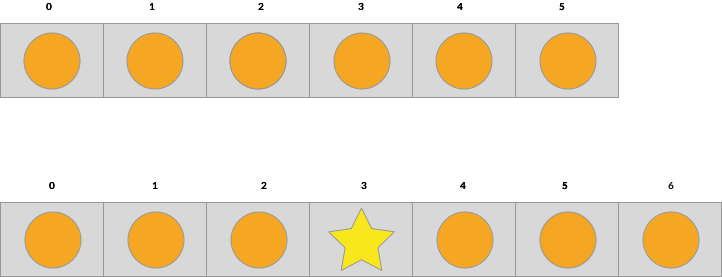
\includegraphics[width=0.8 \linewidth]{images/worksheet_11_q1b_notes.png}
        \end{center}

        to position an element at index $i = 3$ of the list, $n - i = 6 - 3 = 3$
        elements must be moved over.

        \bigskip

        Using this fact, we can generalize that to position an element at index $i$
        of the list, $n - i$ many elements must be shifted.

        \item Learned that when items shifts, it shifts into the expansion room.

        \begin{center}
        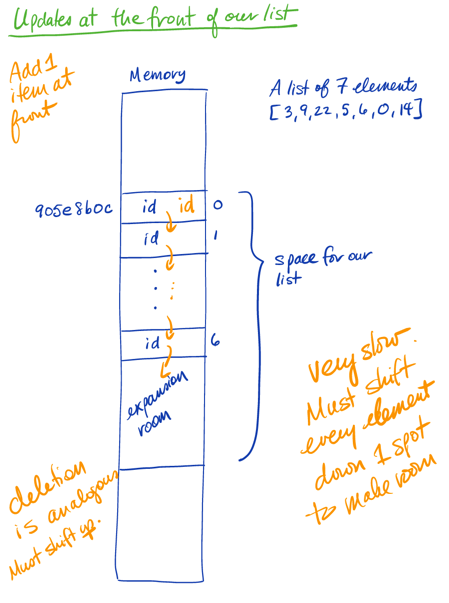
\includegraphics[width=0.8 \linewidth]{images/worksheet_11_q1b_notes2.png}
        \end{center}
    \end{itemize}

    \item Because we know the list size stays as is when an element is removed, we can
    conclude 0 many list elements must be moved.

    \bigskip

    \begin{mdframed}
        \underline{\textbf{Correct Solution:}}

        \color{red}
        The following example tells us

        \begin{center}
        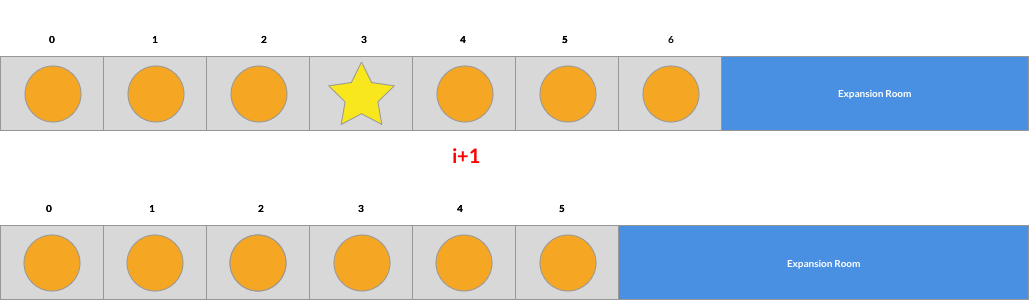
\includegraphics[width=\linewidth]{images/worksheet_11_q1c_correction.png}
        \end{center}

        when an element at index $i = 3$ is removed from the list $n - (i+1) =
        7 - (3 - 1) = 3$ many elements must be moved.

        \bigskip

        Using this fact, we can generalize that when an element is removed,
        $n - (i+1) = n - i - 1$ many elements must be shifted to left.

        \color{black}

    \end{mdframed}

    \item

    \begin{enumerate}[i.]
        \item

        A solution is \textit{LIST.remove(...)}.

        \bigskip

        The answer to question 1.d tells us when an element is removed, $n-i$
        must be shifted to left.

        \bigskip

        Using this fact, we can write a list of smaller size needs to shift elements less.

        \bigskip

        Then, it follows from this fact that $n = 100$ works faster than $n = 1,000,000$.

        \item

        A solution is \textit{LIST.append(...)}

        \bigskip

        The definition of append tells us that upon call, an element is added to
        the end of a list, it takes a constant time to add an element
        as long as the expansion room is not filled.

        \bigskip

        It follows from this fact that $n = 100$ and $n = 1,000,000$ takes roughly
        the same amount of time.
    \end{enumerate}

    \item

    The definition of \textit{Queue} tells us \textit{Queue} is FIFO. That is,
    the first element inserted is the first to come out.

    \bigskip

    Since we know the front of \textit{Queue} is the front of the list, we
    can conclude \textit{LIST.insert(...)} and \textit{LIST.pop(0)} are used
    to support \textit{QUEUE.enqueue} and \textit{QUEUE.dequeue}, respectively.

    \bigskip

    Since we know \textit{LIST.insert(...)} requires shifting of elements by $n - i = n - 0 = n$
    and \textit{LIST.pop(0)} requires shifting of $n - i - 1 = n - 1$ many elements,
    we can conclude both \textit{QUEUE.enqueue} and \textit{QUEUE.dequeue} takes
    longer time as size increases.

    \bigskip

    \begin{mdframed}
        \underline{\textbf{Correct Solution:}}

        The definition of \textit{Queue} tells us \textit{Queue} is FIFO. That is,
        the first element inserted is the first to come out.

        \bigskip

        Since we know the front of \textit{Queue} is the front of the list, we
        can conclude \color{red}\textit{LIST.append(...)}\color{black}\:and \color{red}\textit{LIST.pop(0)}\color{black}\:are used
        to support \textit{QUEUE.enqueue} and \textit{QUEUE.dequeue}, respectively.

        \bigskip

        Since we know \color{red}\textit{LIST.append(...)}\color{black}\:requires the shifting of elements by $n - i = n - n = 0$
        and \textit{LIST.pop(0)} requires shifting of $n - i - 1 = n - 1$ many elements,
        we can conclude \textit{QUEUE.dequeue} takes longer time as size increases.

    \end{mdframed}

    \bigskip

    \underline{\textbf{Notes:}}

    \bigskip

    \begin{itemize}
        \item Learned that the \textbf{front of queue} is where \textit{QUEUE.dequeue}
        occurs.

        \begin{center}
        
\includegraphics[width=0.8 \linewidth]{images/worksheet_11_q1e_notes.png}
        \end{center}
    \end{itemize}

\end{enumerate}

\section*{Question 2 }
\begin{enumerate}[a.]
    \item

    \underline{\textbf{Stack 1:}}

    \bigskip

    \begin{align*}
        \text{Number of steps for \textit{s.push(1)}} + \text{Number of steps for \textit{s.pop()}} &= 1 + 1\\
        &= 2
    \end{align*}

    \bigskip

    \underline{\textbf{Stack 2:}}

    \bigskip

    \begin{align*}
        \text{Number of steps for \textit{s.push(1)}} + \text{Number of steps for \textit{s.pop()}} &= (n+1) + (n+1)\\
        &= 2n + 1
    \end{align*}

    \item

    \underline{\textbf{Stack 1:}}

    \bigskip

    We need to determine the total number of steps taken in the code using \textit{Stack 1}.

    \bigskip

    First, we need to find the number of steps taken per iteration.

    \bigskip

    The code tells us there is only \textit{s.push(i)} in for loop.

    \bigskip

    Since we know the \textit{push} operation in \textit{Stack 1} takes 1 step,
    we can conclude 1 step is taken per iteration.

    \bigskip

    Finally, we need to determine the total number of steps taken.

    \bigskip

    Because we know the loop performs 5 iterations and each iteration takes 1 step,
    we can conclude the code takes total of

    \begin{align}
        5 \cdot 1 = 5
    \end{align}

    steps.

    \bigskip

    \underline{\textbf{Stack 2:}}

    \bigskip

    We need to determine the total number of steps taken in the code using \textit{Stack 2}.

    \bigskip

    First, we need to find the number of steps taken per iteration.

    \bigskip

    The code tells us there is only \textit{s.push(i)} in for loop.

    \bigskip

    Since we know the list in $s$ starts empty, and the size of list grows to $i$ at $i^{th}$
    iteration, we can conclude the size of list $n$ is $i$.

    \bigskip

    Since we know the \textit{push} operation in \textit{Stack 2} takes $n+1$ step,
    and since we know $n = i$, we can conclude $i+1$ step is taken per iteration.

    \bigskip

    Finally, we need to determine the total number of steps taken.

    \bigskip

    Because we know the loop starts at $i = 0$, ends at $i = 4$ with each iteration
    taking $i+1$ steps, we can conclude the code has total of

    \setcounter{equation}{0}
    \begin{align}
        \sum\limits_{i=0}^4 (i+1) &= \sum\limits_{i'=1}^5 i'\\
        &= \frac{5(5+1)}{2}\\
        &= \frac{30}{2}\\
        &= 15
    \end{align}

    steps.


    \item

    \underline{\textbf{Stack 1:}}

    \bigskip

    We need to determine the total number of steps taken in the code using \textit{Stack 1}.

    \bigskip

    First, we need to find the number of steps taken per iteration.

    \bigskip

    The code tells us there is only \textit{s.push(i)} in for loop.

    \bigskip

    Since we know the \textit{push} operation in \textit{Stack 1} takes 1 step,
    we can conclude 1 step is taken per iteration.

    \bigskip

    Finally, we need to determine the total number of steps taken.

    \bigskip

    Because we know the loop performs $(k-1) - 0 + 1 = k$ iterations and each
    iteration takes 1 step, we can conclude the code takes total of

    \begin{align}
        k \cdot 1 = k
    \end{align}

    steps.

    \bigskip

    \underline{\textbf{Stack 2:}}

    \bigskip

    We need to determine the total number of steps taken in the code using \textit{Stack 2}.

    \bigskip

    First, we need to find the number of steps taken per iteration.

    \bigskip

    The code tells us there is only \textit{s.push(i)} in for loop.

    \bigskip

    Since we know the list in $s$ starts empty, and the size of list grows to $i$ at $i^{th}$
    iteration, we can conclude the size of list $n$ is $i$.

    \bigskip

    Since we know the \textit{push} operation in \textit{Stack 2} takes $n+1$ step,
    and since we know $n = i$, we can conclude $i+1$ step is taken per iteration.

    \bigskip

    Finally, we need to determine the total number of steps taken.

    \bigskip

    Because we know the loop starts at $i = 0$, ends at $i = k-1$ with each iteration
    taking $i+1$ steps, we can conclude the code has total of

    \setcounter{equation}{0}
    \begin{align}
        \sum\limits_{i=0}^{k-1} (i+1) &= \sum\limits_{i'=1}^k i'\\
        &= \frac{k(k+1)}{2}
    \end{align}

    steps.

    \bigskip

    \begin{mdframed}
        \underline{\textbf{Correct Solution:}}

        \bigskip

        \underline{\textbf{Stack 1:}}

        \bigskip

        We need to determine the total number of steps taken in the code using \textit{Stack 1}.

        \bigskip

        First, we need to find the number of steps taken per iteration.

        \bigskip

        The code tells us there is only \textit{s.push(i)} in for loop.

        \bigskip

        Since we know the \textit{push} operation in \textit{Stack 1} takes 1 step,
        we can conclude 1 step is taken per iteration.

        \bigskip

        Finally, we need to determine the total number of steps taken.

        \bigskip

        Because we know the loop performs $(k-1) - 0 + 1 = k$ iterations and each
        iteration takes 1 step, we can conclude the code takes total of
        \color{red}
        \setcounter{equation}{0}
        \begin{align}
            k \cdot 1 = k
        \end{align}
        \color{black}

        steps.

        \bigskip

        \underline{\textbf{Stack 2:}}

        \bigskip

        We need to determine the total number of steps taken in the code using \textit{Stack 2}.

        \bigskip

        First, we need to find the number of steps taken per iteration.

        \bigskip

        The code tells us there is only \textit{s.push(i)} in for loop.

        \bigskip

        Since we know the list in $s$ starts empty, and the size of list grows to $i$ at $i^{th}$
        iteration, we can conclude the size of list $n$ is $i$.

        \bigskip

        Since we know the \textit{push} operation in \textit{Stack 2} takes $n+1$ step,
        and since we know $n = i$, we can conclude $i+1$ step is taken per iteration.

        \bigskip

        Finally, we need to determine the total number of steps taken.

        \bigskip

        Because we know the loop starts at $i = 0$, ends at $i = k-1$ with each iteration
        taking $i+1$ steps, we can conclude the code has total of

        \setcounter{equation}{0}
        \begin{align}
            \sum\limits_{i=0}^{k-1} (i+1) &= \sum\limits_{i'=1}^k i'\\
            &= \frac{k(k+1)}{2}
        \end{align}

        steps.

    \end{mdframed}

    \item

    \underline{\textbf{Stack 1:}}

    \bigskip

    We need to determine the total number of steps taken using \textit{Stack 1}.

    \bigskip

    First, we need to determine the number of steps taken by \textit{s2.push(s1.pop())}.

    \bigskip

    The problem tells us both \textit{s2.push(...)} and \textit{s1.pop()} takes 1 step.

    \bigskip

    Using this fact, we can conclude \textit{s2.push(s1.pop())} takes 1 step.

    \bigskip

    Second, we need to determine the total number of steps taken by loop 1.

    \bigskip

    The code tells us that for loop 1, an element popped from \textit{s1} is inserted to \textit{s2},
    and this is repeated until no elements are left in \textit{s1}.

    \bigskip

    Since we know \textit{s1} starts with $n$ many elements, and its size decreases
    by 1 until its length is 0, we can write that with $k$ representing
    $k^{th}$ iteration in loop 1, the terminating condition is reached when

    \setcounter{equation}{0}
    \begin{align}
        n - k &\leq 0\\
        n &\leq k
    \end{align}

    \bigskip

    Since we are looking for the smallest value of $k$ (because it represents
    the number of iterations), we can conclude loop 1 has

    \begin{align}
        \lceil n \rceil = n
    \end{align}

    many iterations.

    \bigskip

    Since we know each iteration in loop 1 takes 1 step, we can conclude
    loop 1 takes total of

    \begin{align}
        n \cdot 1 = n
    \end{align}

    steps.

    \bigskip

    Third, we need to show that the second loop takes total of 0 steps.

    \bigskip

    The code tells us \textit{s2} starts a stack of size 0.

    \bigskip

    Since we know loop 2 doesn't run when the size of stack in \textit{s2} is 0,
    we can conclude loop 2 has 0 iterations.

    \bigskip

    Using this fact, we can conclude loop 2 has total of 0 steps.

    \bigskip

    Finally, we need to determine the total number of steps taken in this code.

    \bigskip

    Since we know loop 1 takes total of $n$ steps and loop 2 takes total of 0 step, we can
    conclude the total number of steps taken by the code is

    \begin{align}
        n + 0 = n
    \end{align}

    steps.

    \bigskip

    % \begin{mdframed}
    %     \underline{\textbf{Rough Work:}}

    %     \bigskip

    %     We need to determine the total number of steps taken using \textit{Stack 1}.

    %     \bigskip

    %     \begin{enumerate}[1.]
    %         \item Determine the number of steps taken by \textit{s2.push(s1.pop())}

    %         \bigskip

    %         First, we need to determine the number of steps taken by \textit{s2.push(s1.pop())}.

    %         \bigskip

    %         \begin{mdframed}

    %         First, we need to determine the number of steps taken by \textit{s2.push(s1.pop())}.

    %         \bigskip

    %         The problem tells us both \textit{s2.push(...)} and \textit{s1.pop()} takes 1 step.

    %         \bigskip

    %         Using this fact, we can conclude \textit{s2.push(s1.pop())} takes 1 step.

    %         \end{mdframed}

    %         \item Determine the total number of steps taken by loop 1.

    %         \bigskip

    %         Second, we need to determine the total number of steps taken by loop 1.

    %         \bigskip

    %         \begin{mdframed}
    %         Second, we need to determine the total number of steps taken by loop 1.

    %         \bigskip

    %         The code tells us that for loop 1, an element popped from \textit{s1} is inserted to \textit{s2},
    %         and this is repeated until no elements are left in \textit{s1}.

    %         \bigskip

    %         Since we know \textit{s1} starts with $n$ many elements, and its size decreases
    %         by 1 until its length is 0, we can write that with $k$ representing
    %         $k^{th}$ iteration in loop 1, the terminating condition is reached when

    %         \begin{align}
    %             n - k &\leq 0\\
    %             n &\leq k
    %         \end{align}

    %         \bigskip

    %         Since we are looking for the smallest value of $k$ (because it represents
    %         the number of iterations), we can conclude loop 1 has

    %         \begin{align}
    %             \lceil n \rceil = n
    %         \end{align}

    %         many iterations.

    %         \bigskip

    %         Since we know each iteration in loop 1 takes 1 step, we can conclude
    %         loop 1 takes total of

    %         \begin{align}
    %             n \cdot 1 = n
    %         \end{align}

    %         steps.

    %         \end{mdframed}

    %         \item Show that the second loop takes total of 0 steps.

    %         \bigskip

    %         Third, we need to show that the second loop takes total of 0 steps.

    %         \bigskip

    %         \begin{mdframed}
    %         Third, we need to show that the second loop takes total of 0 steps.

    %         \bigskip

    %         The code tells us \textit{s2} starts a stack of size 0.

    %         \bigskip

    %         Since we know loop 2 doesn't run when the size of stack in \textit{s2} is 0,
    %         we can conclude loop 2 has 0 iterations.

    %         \bigskip

    %         Using this fact, we can conclude loop 2 has total of 0 steps.

    %         \end{mdframed}

    %         \item Calculate the total number of steps.

    %         \begin{mdframed}
    %         Finally, we need to determine the total number of steps taken in this code.

    %         \bigskip

    %         Since we know loop 1 takes total of $n$ steps and loop 2 takes total of 0 step, we can
    %         conclude the total number of steps taken by the code is

    %         \begin{align}
    %             n + 0 = n
    %         \end{align}

    %         steps.

    %         \end{mdframed}

    %     \end{enumerate}

    %     \bigskip

    %     \begin{mdframed}

    %     \underline{\textbf{Stack 1:}}

    %     \bigskip

    %     We need to determine the total number of steps taken using \textit{Stack 1}.

    %     \bigskip

    %     First, we need to determine the number of steps taken by \textit{s2.push(s1.pop())}.

    %     \bigskip

    %     The problem tells us both \textit{s2.push(...)} and \textit{s1.pop()} takes 1 step.

    %     \bigskip

    %     Using this fact, we can conclude \textit{s2.push(s1.pop())} takes 1 step.

    %     \bigskip

    %     Second, we need to determine the total number of steps taken by loop 1.

    %     \bigskip

    %     The code tells us that for loop 1, an element popped from \textit{s1} is inserted to \textit{s2},
    %     and this is repeated until no elements are left in \textit{s1}.

    %     \bigskip

    %     Since we know \textit{s1} starts with $n$ many elements, and its size decreases
    %     by 1 until its length is 0, we can write that with $k$ representing
    %     $k^{th}$ iteration in loop 1, the terminating condition is reached when

    %     \begin{align}
    %         n - k &\leq 0\\
    %         n &\leq k
    %     \end{align}

    %     \bigskip

    %     Since we are looking for the smallest value of $k$ (because it represents
    %     the number of iterations), we can conclude loop 1 has

    %     \begin{align}
    %         \lceil n \rceil = n
    %     \end{align}

    %     many iterations.

    %     \bigskip

    %     Since we know each iteration in loop 1 takes 1 step, we can conclude
    %     loop 1 takes total of

    %     \begin{align}
    %         n \cdot 1 = n
    %     \end{align}

    %     steps.

    %     \bigskip

    %     Third, we need to show that the second loop takes total of 0 steps.

    %     \bigskip

    %     The code tells us \textit{s2} starts a stack of size 0.

    %     \bigskip

    %     Since we know loop 2 doesn't run when the size of stack in \textit{s2} is 0,
    %     we can conclude loop 2 has 0 iterations.

    %     \bigskip

    %     Using this fact, we can conclude loop 2 has total of 0 steps.

    %     \bigskip

    %     Finally, we need to determine the total number of steps taken in this code.

    %     \bigskip

    %     Since we know loop 1 takes total of $n$ steps and loop 2 takes total of 0 step, we can
    %     conclude the total number of steps taken by the code is

    %     \begin{align}
    %         n + 0 = n
    %     \end{align}

    %     steps.

    %     \end{mdframed}

    % \end{mdframed}

    \bigskip

    \underline{\textbf{Stack 2:}}

    \bigskip

    We need to determine the total number of steps taken using \textit{Stack 2}.

    \bigskip

    First, we need to determine the number of steps taken by \textit{s2.push(s1.pop())} in loop 1.

    \bigskip

    The code tells us that \textit{s1.pop()} operation takes $n_1 + 1$ steps and
    \textit{s2.push(...)} takes $n_2 + 1$ steps, where $n_1$ and $n_2$
    be the size of stack for \textit{s1} and \textit{s2}, respectively.

    \bigskip

    Since we know $s2$ starts as an empty stack, and $s1$ starts as a stack
    with the size of $n$, and since we know \textit{s2.push()} and \textit{s1.pop(...)} causes the
    stack size of \textit{s2} and \textit{s1} to increase and decrease by 1 per iteration, respectively,
    we can conclude that at $k^{th}$ iteration, \textit{s2.push(s1.pop())}
    takes total of

    \begin{align}
        (n - k + 1) + (k + 1) = n + 2
    \end{align}

    steps.

    \bigskip

    Second, we need to determine the total number of steps taken by loop 1.

    \bigskip

    The code tells us that for loop 1, an element popped from \textit{s1} is inserted to \textit{s2},
    and this is repeated until no elements are left in \textit{s1}.

    \bigskip

    Since we know \textit{s1} starts with $n$ many elements, and its size decreases
    by 1 until its length is 0, we can write that with $k$ representing
    $k^{th}$ iteration in loop 1, the terminating condition is reached when

    \begin{align}
        n - k &\leq 0\\
        n &\leq k
    \end{align}

    \bigskip

    Since we are looking for the smallest value of $k$ (because it represents
    the number of iterations), we can conclude loop 1 has

    \begin{align}
        \lceil n \rceil = n
    \end{align}

    many iterations.

    \bigskip

    Since we know each iteration in loop 1 takes $n+2$ step, we can conclude
    loop 1 takes total of

    \begin{align}
        n \cdot (n+2) = n(n+2)
    \end{align}

    steps.

    \bigskip

    Third, we need to show that the second loop takes total of 0 steps.

    \bigskip

    The code tells us \textit{s2} starts a stack of size 0.

    \bigskip

    Since we know loop 2 doesn't run when the size of stack in \textit{s2} is 0,
    we can conclude loop 2 has 0 iterations.

    \bigskip

    Using this fact, we can conclude loop 2 has total of 0 steps.

    \bigskip

    Finally, we need to determine the total number of steps taken in this code.

    \bigskip

    Since we know loop 1 takes total of $n$ steps and loop 2 takes total of 0 step, we can
    conclude the total number of steps taken by the code is

    \begin{align}
        n(n+2) + 0 = n(n+2)
    \end{align}

    steps.

    % \begin{mdframed}
    %     \underline{\textbf{Rough Work:}}

    %     \bigskip

    %     We need to determine the total number of steps taken using \textit{Stack 2}.

    %     \bigskip

    %     \begin{enumerate}[1.]
    %         \item Determine the number of steps taken by \textit{s2.push(s1.pop())} in loop 1.

    %         \bigskip

    %         First, we need to determine the number of steps taken by \textit{s2.push(s1.pop())} in loop 1.

    %         \bigskip

    %         \begin{enumerate}[1.]
    %             \item State that \textit{s1.pop()} takes $n_1 + 1$ steps and \textit{s2.push(...)}
    %             takes $n_2 + 1$.

    %             \begin{mdframed}
    %             The code tells us that \textit{s1.pop()} operation takes $n_1 + 1$ steps and
    %             \textit{s2.push(...)} takes $n_2 + 1$ steps, where $n_1$ and $n_2$ be the size of stack for \textit{s1}
    %             and \textit{s2}, respectively..
    %             \end{mdframed}

    %             \item Show that \textit{s2.push(s1.pop())} takes $i + 2$ steps.

    %             \begin{mdframed}
    %             Since we know $s2$ starts as an empty stack, and $s1$ starts as a stack
    %             with the size of $n$, and since we know \textit{s2.push()} and \textit{s1.pop(...)} causes the
    %             stack size of \textit{s2} and \textit{s1} to increase and decrease by 1 per iteration, respectively,
    %             we can conclude that at $k^{th}$ iteration, \textit{s2.push(s1.pop())}
    %             takes total of

    %             \begin{align}
    %                 (n - k + 1) + (k + 1) = n + 2
    %             \end{align}

    %             steps.

    %             \end{mdframed}
    %         \end{enumerate}

    %         \bigskip

    %         \begin{mdframed}
    %         First, we need to determine the number of steps taken by \textit{s2.push(s1.pop())} in loop 1.

    %         \bigskip

    %         The code tells us that \textit{s1.pop()} operation takes $n_1 + 1$ steps and
    %         \textit{s2.push(...)} takes $n_2 + 1$ steps, where $n_1$ and $n_2$
    %         be the size of stack for \textit{s1} and \textit{s2}, respectively.

    %         \bigskip

    %         Since we know $s2$ starts as an empty stack, and $s1$ starts as a stack
    %         with the size of $n$, and since we know \textit{s2.push()} and \textit{s1.pop(...)} causes the
    %         stack size of \textit{s2} and \textit{s1} to increase and decrease by 1 per iteration, respectively,
    %         we can conclude that at $k^{th}$ iteration, \textit{s2.push(s1.pop())}
    %         takes total of

    %         \begin{align}
    %             (n - k + 1) + (k + 1) = n + 2
    %         \end{align}

    %         steps.

    %         \end{mdframed}

    %         \item Determine the total number of steps taken by loop 1.

    %         \bigskip

    %         Second, we need to determine the total number of steps taken by loop 1.

    %         \bigskip

    %         \begin{enumerate}[1.]
    %             \item State that for loop 1, an element popped from \textit{s1}
    %             is inserted to \textit{s2}, and this is repeated until no elements are left in \textit{s1}.

    %             \begin{mdframed}
    %             The code tells us that for loop 1, an element popped from \textit{s1} is inserted to \textit{s2},
    %             and this is repeated until no elements are left in \textit{s1}.
    %             \end{mdframed}

    %             \item Show loop 1 takes $n$ iterations.

    %             \begin{mdframed}
    %             Since we know \textit{s1} starts with $n$ many elements, and its size decreases
    %             by 1 until its length is 0, we can write that with $k$ representing
    %             $k^{th}$ iteration in loop 1, the terminating condition is reached when

    %             \begin{align}
    %                 n - k &\leq 0\\
    %                 n &\leq k
    %             \end{align}

    %             \bigskip

    %             Since we are looking for the smallest value of $k$ (because it represents
    %             the number of iterations), we can conclude loop 1 has

    %             \begin{align}
    %                 \lceil n \rceil = n
    %             \end{align}

    %             many iterations.
    %             \end{mdframed}

    %             \item Show loop 1 takes total of $n(n+2)$ steps.

    %             \begin{mdframed}
    %             Since we know each iteration in loop 1 takes $n+2$ step, we can conclude
    %             loop 1 takes total of

    %             \begin{align}
    %                 n \cdot (n+2) = n(n+2)
    %             \end{align}

    %             steps.
    %             \end{mdframed}
    %         \end{enumerate}

    %         \bigskip

    %         \begin{mdframed}
    %         Second, we need to determine the total number of steps taken by loop 1.

    %         \bigskip

    %         The code tells us that for loop 1, an element popped from \textit{s1} is inserted to \textit{s2},
    %         and this is repeated until no elements are left in \textit{s1}.

    %         \bigskip

    %         Since we know \textit{s1} starts with $n$ many elements, and its size decreases
    %         by 1 until its length is 0, we can write that with $k$ representing
    %         $k^{th}$ iteration in loop 1, the terminating condition is reached when

    %         \begin{align}
    %             n - k &\leq 0\\
    %             n &\leq k
    %         \end{align}

    %         \bigskip

    %         Since we are looking for the smallest value of $k$ (because it represents
    %         the number of iterations), we can conclude loop 1 has

    %         \begin{align}
    %             \lceil n \rceil = n
    %         \end{align}

    %         many iterations.

    %         \bigskip

    %         Since we know each iteration in loop 1 takes $n+2$ step, we can conclude
    %         loop 1 takes total of

    %         \begin{align}
    %             n \cdot (n+2) = n(n+2)
    %         \end{align}

    %         steps.

    %         \end{mdframed}

    %         \item Show that the total number of steps taken by loop 2 is 0.

    %         \bigskip

    %         \begin{mdframed}
    %         Third, we need to show that the second loop takes total of 0 steps.

    %         \bigskip

    %         The code tells us \textit{s2} starts a stack of size 0.

    %         \bigskip

    %         Since we know loop 2 doesn't run when the size of stack in \textit{s2} is 0,
    %         we can conclude loop 2 has 0 iterations..

    %         \bigskip

    %         Using this fact, we can conclude loop 2 has total of 0 steps.
    %         \end{mdframed}

    %         \item Conclude by calculating the total number of steps taken in this code.

    %         \begin{mdframed}
    %         Finally, we need to determine the total number of steps taken in this code.

    %         \bigskip

    %         Since we know loop 1 takes total of $n$ steps and loop 2 takes total of 0 step, we can
    %         conclude the total number of steps taken by the code is

    %         \begin{align}
    %             n(n+2) + 0 = n(n+2)
    %         \end{align}

    %         steps.
    %         \end{mdframed}
    %     \end{enumerate}

        % \bigskip

    %     \begin{mdframed}

    %     \underline{\textbf{Stack 2:}}

    %     \bigskip

    %     We need to determine the total number of steps taken using \textit{Stack 2}.

    %     \bigskip

    %     First, we need to determine the number of steps taken by \textit{s2.push(s1.pop())} in loop 1.

    %     \bigskip

    %     The code tells us that \textit{s1.pop()} operation takes $n_1 + 1$ steps and
    %     \textit{s2.push(...)} takes $n_2 + 1$ steps, where $n_1$ and $n_2$
    %     be the size of stack for \textit{s1} and \textit{s2}, respectively.

    %     \bigskip

    %     Since we know $s2$ starts as an empty stack, and $s1$ starts as a stack
    %     with the size of $n$, and since we know \textit{s2.push()} and \textit{s1.pop(...)} causes the
    %     stack size of \textit{s2} and \textit{s1} to increase and decrease by 1 per iteration, respectively,
    %     we can conclude that at $k^{th}$ iteration, \textit{s2.push(s1.pop())}
    %     takes total of

    %     \begin{align}
    %         (n - k + 1) + (k + 1) = n + 2
    %     \end{align}

    %     steps.

    %     \bigskip

    %     Second, we need to determine the total number of steps taken by loop 1.

    %     \bigskip

    %     The code tells us that for loop 1, an element popped from \textit{s1} is inserted to \textit{s2},
    %     and this is repeated until no elements are left in \textit{s1}.

    %     \bigskip

    %     Since we know \textit{s1} starts with $n$ many elements, and its size decreases
    %     by 1 until its length is 0, we can write that with $k$ representing
    %     $k^{th}$ iteration in loop 1, the terminating condition is reached when

    %     \begin{align}
    %         n - k &\leq 0\\
    %         n &\leq k
    %     \end{align}

    %     \bigskip

    %     Since we are looking for the smallest value of $k$ (because it represents
    %     the number of iterations), we can conclude loop 1 has

    %     \begin{align}
    %         \lceil n \rceil = n
    %     \end{align}

    %     many iterations.

    %     \bigskip

    %     Since we know each iteration in loop 1 takes $n+2$ step, we can conclude
    %     loop 1 takes total of

    %     \begin{align}
    %         n \cdot (n+2) = n(n+2)
    %     \end{align}

    %     steps.

    %     \bigskip

    %     Third, we need to show that the second loop takes total of 0 steps.

    %     \bigskip

    %     The code tells us \textit{s2} starts a stack of size 0.

    %     \bigskip

    %     Since we know loop 2 doesn't run when the size of stack in \textit{s2} is 0,
    %     we can conclude loop 2 has 0 iterations.

    %     \bigskip

    %     Using this fact, we can conclude loop 2 has total of 0 steps.

    %     \bigskip

    %     Finally, we need to determine the total number of steps taken in this code.

    %     \bigskip

    %     Since we know loop 1 takes total of $n$ steps and loop 2 takes total of 0 step, we can
    %     conclude the total number of steps taken by the code is

    %     \begin{align}
    %         n(n+2) + 0 = n(n+2)
    %     \end{align}

    %     steps.

    %     \end{mdframed}
    % \end{mdframed}

\end{enumerate}

\end{document}